\documentclass[a4paper,11pt]{article}
\author{ 杨旭鹏  \  PB17000234}
\date{2019年秋季}
\title{计算物理A 第八题}

\usepackage{ctex}
\usepackage{amsmath}
\usepackage{amsfonts}
\usepackage{graphicx}
\usepackage{epstopdf}
\usepackage{lastpage}
\usepackage{hyperref}
\usepackage{listings}
\RequirePackage{xcolor}
\usepackage{appendix}
\usepackage{caption2}
\usepackage{subfigure}
\usepackage{float}
\makeatletter\def\@captype{table}\makeatother

\definecolor{dkgreen}{rgb}{0,0.6,0}
\definecolor{gray}{rgb}{0.5,0.5,0.5}
\definecolor{mauve}{rgb}{0.58,0,0.82}

\lstset{
  frame=tb,
  aboveskip=3mm,
  belowskip=3mm,
  showstringspaces=false,
  columns=flexible,
  framerule=1pt,
  rulecolor=\color{gray!35},
  backgroundcolor=\color{gray!5},
  basicstyle={\small\ttfamily},
  numbers=left,
  numberstyle=\tiny\color{gray},
  keywordstyle=\color{blue},
  commentstyle=\color{dkgreen},
  stringstyle=\color{mauve},
  breaklines=true,
  breakatwhitespace=true,
  tabsize=3,            
  }



\begin{document}
\maketitle

\section{题目描述}
用Monte Carlo方法计算如下定积分,并讨论有效数字位数。
\begin{equation}
\int^{2}_{0}dx\sqrt{x+\sqrt{x}}
\end{equation}

\begin{equation}
\int^{0.9}_{0}dx\int^{0.8}_{0}dy\int^{0.9}_{0}dz\int^{2}_{0}du\int^{1.3}_{0}dv (6-x^{2}-y^{2}-z^{2}-u^{2}-v^{2})
\end{equation}



\section{算法}
\subsection{第一个积分}
对于第一个积分,我们可以直接利用Monte Carlo 方法进行计算,即:
\begin{equation}
	\int^{2}_{0}\sqrt{x+\sqrt{x}}dx = 2\left<  \sqrt{x+\sqrt{x}} \right> \doteq \frac{2}{N} \sum  _{i=1}^{N} \sqrt{x_{i}+\sqrt{x_{i}}}
\end{equation}
其中$x_{i}$为在$[0,2]$中均匀抽样得到的数据点。但由于第一个积分式的积分函数并不是很平滑,故可能积分精确度不高,我们可取$g(x)  = \sqrt{x}+\sqrt[4]{x}$将积分转化为$\int^{2}_{0}\frac{f(x)}{g(x)}g(x)dx$。(其中$f(x) = \sqrt{x+\sqrt{x}}$)则对于$\frac{f(x)}{g(x)}$部分来说,其在$[0,2]$之间比较平缓,且接近于1:

\begin{figure}[!htbp]   
\centering     
\subfigure[不平滑的$\sqrt{x+\sqrt{x}}$]{
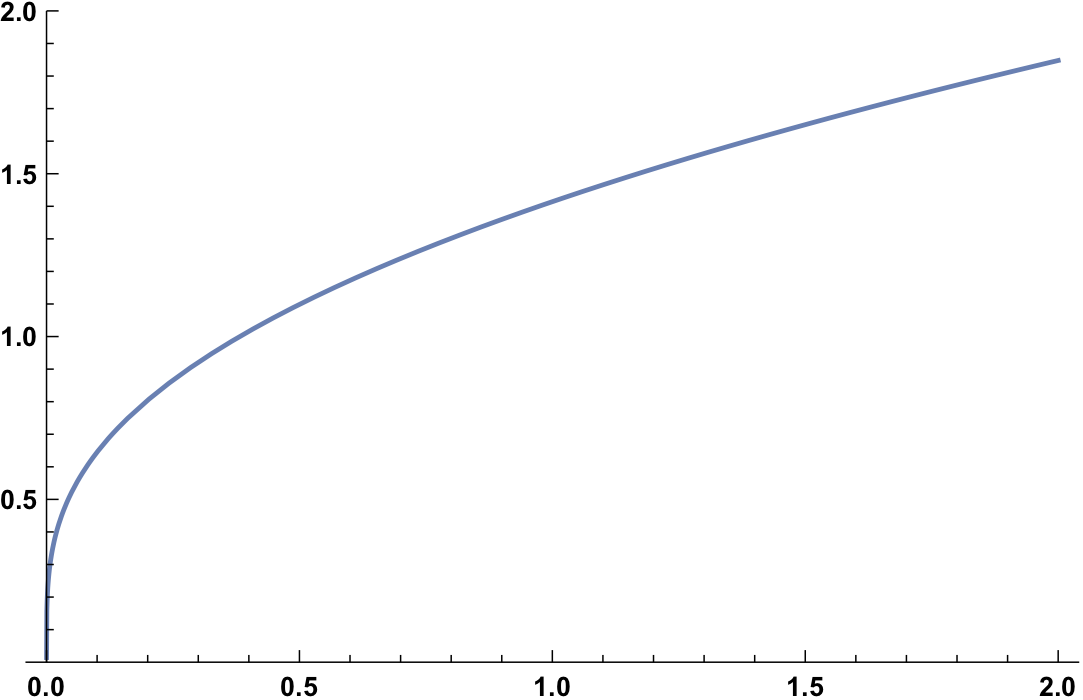
\includegraphics[width=6cm] {f(x).png}
}
\subfigure[相对平滑的$\frac{f(x)}{g(x)}$]{
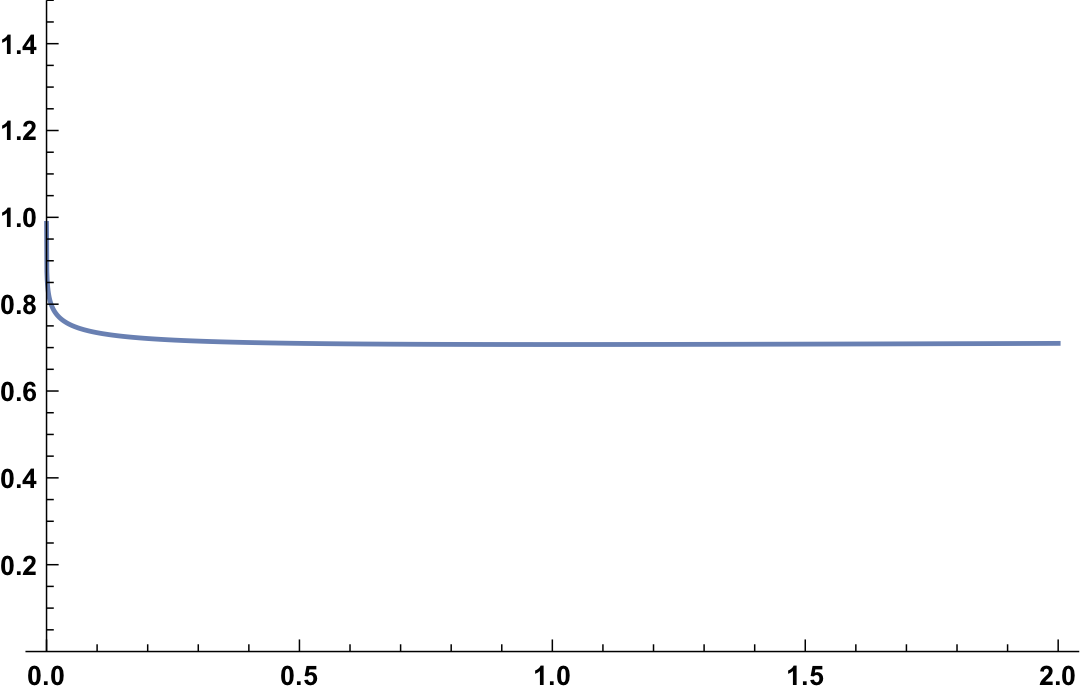
\includegraphics[width=6cm] {fg.png}
}      
\caption{函数示意图}      
\end{figure}



\newpage
而对于$g(x)$来说,我们很容易能计算出其在$[0,2]$上的积分为$\frac{4}{15} \times 2^{\frac{1}{4}} (6 + 5\times 2^{\frac{1}{4}}) \doteq 3.788349467$。则利用权重 Monte Carlo 积分,我们有:
\begin{equation}
\left\{
\begin{array}{l}
	\int^{2}_{0}\frac{f(x)}{g(x)}g(x)dx = \int_{0}^{c}\frac{f(y)}{g(y)}dy \\
	y = \int_{0}^{x} g(t)dt \\
	c = \int_{0}^{2} g(x)dx = \frac{4}{15} \times 2^{\frac{1}{4}} (6 + 5\times 2^{\frac{1}{4}}) \doteq 3.788349467

\end{array}
\right.
\end{equation}
其中选择$y$在$[0,c]$中均匀分布。
则其数值近似解为:
\begin{equation}
	\int^{2}_{0}f(x)dx = \int_{0}^{c}\frac{f(y)}{g(y)}dy = c\left <\frac{f(y)}{g(y)} \right> \doteq \frac{c}{N}\sum _{i=1}^{N}\frac{f(y_{i})}{g(y_{i})}
\end{equation}


\subsection{第二个积分}
我们可直接利用 Monte Carlo 方法进行计算,即:
\begin{equation}
\begin{aligned}
	&\int^{0.9}_{0}dx\int^{0.8}_{0}dy\int^{0.9}_{0}dz\int^{2}_{0}du\int^{1.3}_{0}dv (6-x^{2}-y^{2}-z^{2}-u^{2}-v^{2}) \\
	&= 0.9\times 0.8\times 0.9\times 2\times 1.3 \left<  6-x^{2}-y^{2}-z^{2}-u^{2}-v^{2}   \right> \\
	&\doteq \frac{0.9\times 0.8\times 0.9\times 2\times 1.3}{N}\sum _{i=1}^{N} (6-x^{2}_{i}-y^{2}_{i}-z^{2}_{i}-u^{2}_{i}-v^{2}_{i})
\end{aligned}
\end{equation}
其中$x_{i},y_{i},z_{i},u_{i},v_{i}$分别为在区间$[0,0.9],[0,0.8],[0,0.9],[0,2],[0,1.3]$间均匀抽样得到的数据点。即可计算出第二个积分式得结果。


\subsection{16807产生器}
16807产生器属于线性同余法产生器的特例。而线性同余法方法为:

\begin{equation}
\begin{aligned}
	I_{n+1} &= (aI_{n} + b) \ mod \ m \\
	x_{n} &= I_{n}/m
\end{aligned}
\label{linear}	
\end{equation}

其中整数$I_{i} \in [0,m-1]$,$a,b,m$为算法中的可调参数,其选取直接影响产生器的质量。选取参数:
\begin{equation}
\left\{
\begin{array}{l}
	a = 7^{5} = 16807 \\
	b = 0 \\
	m = 2^{31}-1 = 2147483647
\end{array}
\right.
\end{equation}

即为所谓的16807产生器。由于直接利用\ref{linear}编写程序时计算$(aI_{n} \ mod \ m )$时很容易造成数据溢出,故采取Schrage方法进行具体编程的实现:

\begin{equation}
	aI_{n} \ mod \ m = \left\{
	\begin{array}{l}
		a(I_{n}\ mod \ q) - r[I_{n}/q],\ \ \ \ \ \ \ \ if \geq 0 \\
		a(I_{n}\ mod \ q) - r[I_{n}/q] + m,\ \ otherwise	
			\end{array}
	\right.
\end{equation}

其中$m=aq+r$,即$q=m/a=127773$,$r=m \ mod \ a=2836$。即可利用此方法产生伪随机数序列。



\section{程序使用方法}
在运行程序后,会看到请求输入积分所需总随机点数的提示,按照提示在后面输入所需要的总随机点数,摁回车继续。然后经过计算在屏幕上给出2个积分的结果。程序输出完这些后会自动退出。
\begin{figure}[!htbp]        
\centering

\includegraphics[width=10cm]{example.png}      
\caption{ 一个典型程序的运行示例}      
\end{figure}


\section{程序结果与讨论}
当输入一些不同的点数时,得到如下结果:

\begin{table}[!htbp]
\centering
\resizebox{\textwidth}{!}{
\begin{tabular}{|c|c|c|c|c|c|c|c|}
\hline

&$N=10^{3}$  &$N=10^{4}$  &$N=10^{5}$  &$N=10^{6}$  &$N=10^{7}$
&$N=10^{8}$ &理论值 \\ \hline

积分1结果(变换) &2.698789 &2.700485 &2.700437 &2.700343 &2.700364 &2.700387
&2.689521 \\ \hline
积分1结果(变换)与精确值差值 &0.009268 &0.010964 &0.010916 &0.010822 &0.010843  &0.010866 & \\ \hline

积分1结果(直接抽样) &2.679132 &2.686411 &2.685039 &2.687622 &2.689306 &2.689497
&2.689521 \\ \hline
积分1结果(直接抽样)与精确值差值 &0.010389 &0.003110 &0.004482 &0.001899 &0.000215  &0.000024 & \\ \hline
积分2结果 &5.654970 &5.663653 &5.648212 &5.644032 &5.645314 &5.643928
&5.64408 \\ \hline
积分2结果与精确值差值 &0.010890 &0.019573 &0.004132 &0.000048 &0.000215  &0.000152 & \\ \hline
\end{tabular}}
\caption{积分结果一览表}
\end{table}


\newpage 可以看出积分1利用变换抽样得到的结果并不收敛于准确值。这可能是由于虽然变换将大部分积分区间内的函数变得比较平缓,但由于靠近积分左端的导数很大,故此变换方法很难收敛。

其与精确值的差别与$\frac{1}{\sqrt{N}}$的比较为(不讨论变换法得到的积分1,下同):

\begin{figure}[!htbp]        
\centering
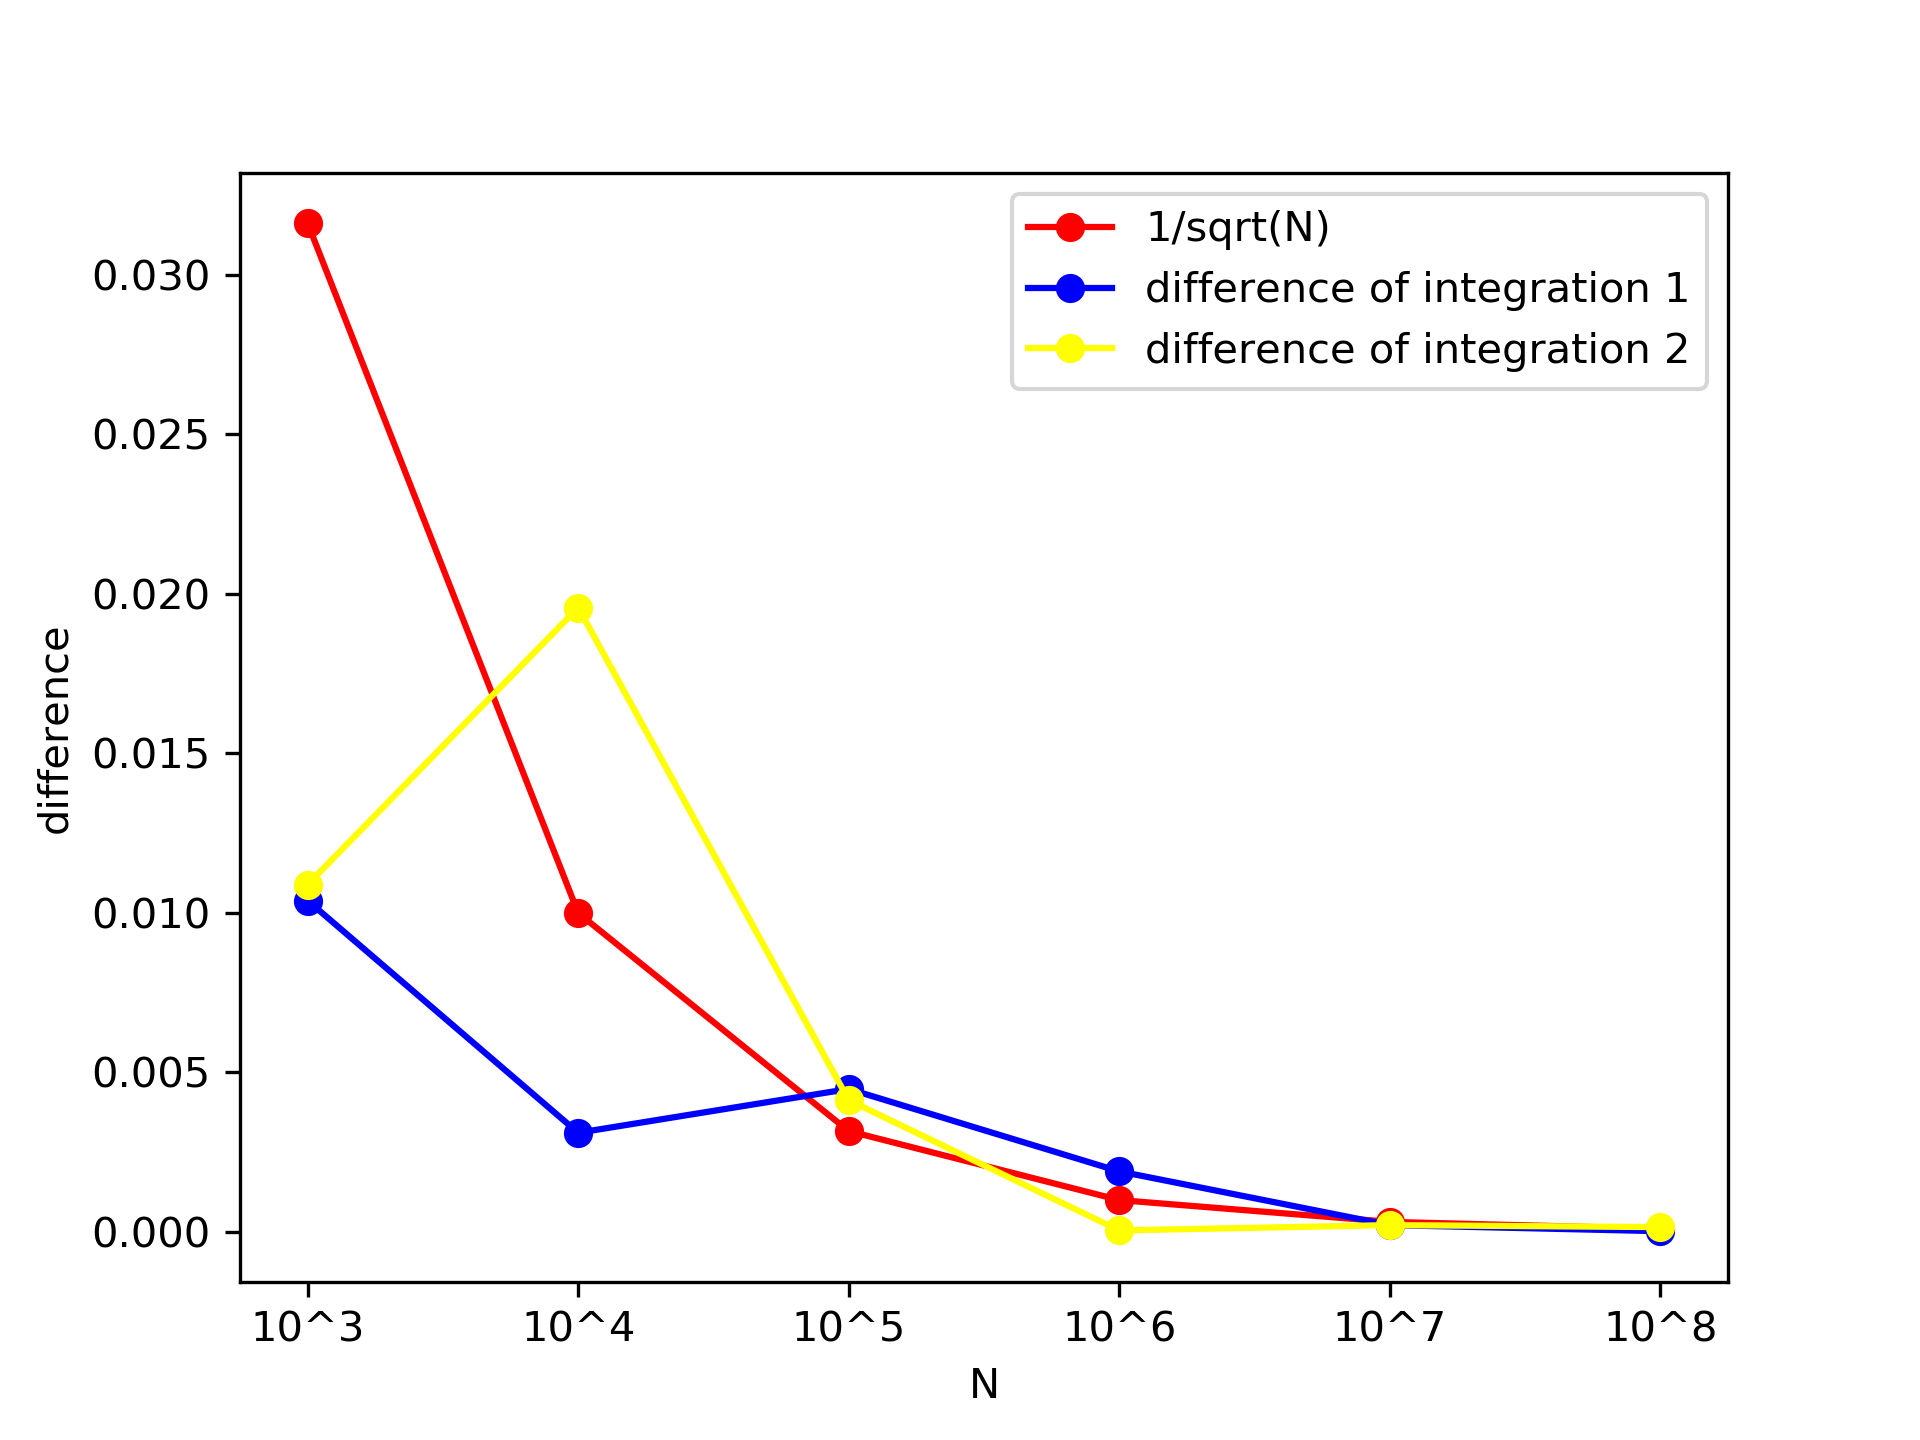
\includegraphics[width=10cm]{difference.png}      
\caption{ 数值积分结果与精确值的差值与$\frac{1}{\sqrt{N}}$的比较}      
\end{figure}

可以看出其数值积分误差与$\frac{1}{\sqrt{N}}$相关。使用不同的种子值得到如下结果:


\begin{table}[!htbp]
\centering
\resizebox{\textwidth}{!}{
\begin{tabular}{|c|c|c|c|c|c|c|}
\hline

&$N=10^{3}$  &$N=10^{4}$  &$N=10^{5}$  &$N=10^{6}$  &$N=10^{7}$
&$N=10^{8}$  \\ \hline

积分1结果与精确值差别1 &0.009551 &0.002047 &0.000933 &0.000084 &0.000036 &0.000039  \\ \hline
积分1结果与精确值差别2 &0.025366 &0.002164 &0.003410 &0.000575 &0.000224 &0.000033  \\ \hline
积分1结果与精确值差别3 &0.000016 &0.003167 &0.001923 &0.000487 &0.000130 &0.000055  \\ \hline
积分1结果与精确值差别4 &0.020162 &0.005893 &0.002752 &0.001050 &0.000066 &0.000085  \\ \hline

积分1结果与精确值差别5 &0.008691 &0.018182 &0.002630 &0.001048 &0.000143 &0.000032  \\ \hline
积分2结果与精确值差别1 &0.035440 &0.021787 &0.000213 &0.000625 &0.000146 &0.000205  \\ \hline

积分2结果与精确值差别2 &0.054598 &0.012395 &0.003819 &0.001073 &0.000821 &0.000162  \\ \hline
积分2结果与精确值差别3 &0.096984 &0.022211 &0.008630 &0.002231 &0.000570 &0.000120  \\ \hline
积分2结果与精确值差别4 &0.060068 &0.006463 &0.000507 &0.000968 &0.000629 &0.000098  \\ \hline
积分2结果与精确值差别5 &0.003673 &0.011706 &0.017530 &0.003387 &0.001163 &0.000100  \\ \hline


\end{tabular}}
\caption{积分结果误差}
\end{table}




\newpage 则可推知其积分有效位数分别为:

\begin{table}[!htbp]
\centering
\resizebox{\textwidth}{!}{
\begin{tabular}{|c|c|c|c|c|c|c|}
\hline

&$N=10^{3}$  &$N=10^{4}$  &$N=10^{5}$  &$N=10^{6}$  &$N=10^{7}$
&$N=10^{8}$  \\ \hline

积分1有效位数 &2 &2 &3 &3 &4 &4  \\ \hline
积分2有效位数 &1 &2 &2 &3 &3 &4  \\ \hline

\end{tabular}}
\caption{积分结果一览表}
\end{table}






\newpage
\section{心得与体会}
通过此次作业,对Monte Carlo 法积分更加熟悉,也对其结果的有效位数有了更深的理解。发现变换法对于有些函数来说即使让其在积分区间内比较平缓,但若出现导数在某点很大时,数值积分结果会相当不好,甚至不收敛。

通过编程作业,也更加熟悉了一些C语言和\LaTeX 。

\newpage
\section{附录}

\begin{appendices}


\section{C语言源程序}
\begin{lstlisting}[language = C]
#include <stdio.h>
#include <stdlib.h>
#include <time.h>
#include <math.h>
#define a 16807
#define b 0
#define m 2147483647
#define r (m%a)
#define q (m/a)
#define Pi 3.1415926



//利用/dev/random 产生"真"随机数
int my_realrandom(int ran[],int n){
    FILE * fp1 = fopen("/dev/random","r");
    for(int i=0;i<n;i++){
        fread(&ran[i], 1, 4, fp1);
    }
    fclose(fp1);
    return 0;
}


// Schrage 方法产生随机数
int my_schrage(double ran[],int seed,int n){
    for (int i = 0; i < n - 1; i++) {
        if (seed >= 0) {
            ran[i] = (seed / (double) m);
        } else {
            ran[i] = ((seed + m) / (double) m);
        }
        if(seed == m-1){
            if(a >=  b){    //由于Schrage方法只对z in (0,m-1)成立,故这里要讨论z == m-1的情况
                seed = m + (b-a) % m;
            }
            else   seed =  (b-a) % m;

        }
        else seed = ((a * (seed % q) - r * (seed /  q)) + b % m ) % m;  //递推式
    }
    if (seed >= 0) {
        ran[n-1] = (seed / (double) m);
    } else {
        ran[n-1] = ((seed + m) / (double) m);
    }
    return 0;
}





int main(int argc, const char * argv[]) {
    int N;    //总随机数个数
    double x1,x2,x3,x4,x5,x6,x7;
    double result1 = 0;
    double result2 = 0;
    double result3 = 0;
    char str[50];
    printf("请输入您计算积分所需要的总点数:");
    while (!scanf("%d",&N)){   //简单的输入检查
        gets(str);
        printf("\nInput error,please try again\n");
        printf("请输入您计算积分所需要的总点数:");
    }
    if(N >1000000) printf("您输入的参数已接受,正在计算请稍等片刻~\n");
    int seed[5];
    my_realrandom(seed,5); //读取"/dev/random"产生随机种子方便多次调用

    double *ran1 = malloc(sizeof(double) * N);  //用来存放随机数
    double *ran2 = malloc(sizeof(double) * N);  //用来存放随机数
    double *ran3 = malloc(sizeof(double) * N);  //用来存放随机数
    double *ran4 = malloc(sizeof(double) * N);  //用来存放随机数
    double *ran5 = malloc(sizeof(double) * N);  //用来存放随机数

    my_schrage(ran1,seed[0],N);
    my_schrage(ran2,seed[1],N);
    my_schrage(ran3,seed[2],N);
    my_schrage(ran4,seed[3],N);
    my_schrage(ran5,seed[4],N);
    
    
    for(int i = 0;i < N;i++){
        x1 = 3.78834946716848*ran1[i];
        x2 = 2*ran1[i];
        x3 = 0.9*ran1[i];
        x4 = 0.8*ran2[i];
        x5 = 0.9*ran3[i];
        x6 = 2*ran4[i];
        x7 = 1.3*ran5[i];
        result1 += 3.78834946716848*sqrt(x1+sqrt(x1))/(sqrt(x1) + sqrt(sqrt(x1)))/N;  //第一个积分变换方法
        result2 += 2*sqrt(x2+sqrt(x2))/N; //第一个积分直接抽样计算法
        result3 += 1.6848*(6-pow(x3,2)-pow(x4,2)-pow(x5,2)-pow(x6,2)-pow(x7,2))/N;  //第二个积分直接抽样计算法
    }
    
    printf("the integation1-1(with transformation) is %lf,the difference is %lf\n",result1,fabs(result1-2.689521));   //第一个积分变换方法
    printf("the integation1-2 is %lf,the difference is %lf\n",result2,fabs(result2-2.689521));  //第一个积分直接抽样计算法
    printf("the integation2-1 is %lf,the difference is %lf\n",result3,fabs(result3-5.64408));  //第二个积分直接抽样计算法
    return 0;
}

\end{lstlisting}

\newpage

\section{可视化绘图python程序源码}

\begin{lstlisting}[language = python]

import matplotlib.pyplot as plt
from mpl_toolkits.mplot3d import Axes3D
import numpy as np
#from IPython.core.pylabtools import figsize # import figsize
#figsize(12.5, 4) # 设置 figsize
plt.rcParams['savefig.dpi'] = 300 #图片像素
plt.rcParams['figure.dpi'] = 300 #分辨率
# 默认的像素:[6.0,4.0],分辨率为100,图片尺寸为 600&400
fig = plt.figure()
ax1 = fig.add_subplot(111)
X = []
Y = []

with open('problem 6/p_108.txt', 'r') as f:
    while True:
        lines = f.readline() # 整行读取数据
        if not lines:
            break
        Y = [float(i) for i in lines.split(',')]  # 将整行数据分割处理
    Y = np.array(Y) # 将数据从list类型转换为array类型。


X = np.arange(-2.995, 3.005, 0.01)

plt.bar(x=X, height=Y, width=0.01, label='actual probability')
ax1.legend(loc=1)
ax1.set_ylabel('probability')


X = np.arange(-2.995, 3.005, 0.01)
oY = 0.01/(1+X**4)/2.196879736
ax1.plot(X, oY, 'r', label='original probability')
ax1.legend(loc=2)
plt.ylim([0,0.0055])
plt.xlabel('X')


plt.savefig("2.png")

\end{lstlisting}


\end{appendices}




\end{document}
